%
% kreis.tex 
%
% (c) 2018 Prof Dr Andreas Müller, Hochschule Rapperswil
%
\section{Kreis und Kugel\label{section:kreisundkugel}}
\rhead{Kreis und Kugel}
Da das Skalarprodukt die Länge eines Vektors berechnet, kann man
jetzt auch die Menge der Punkte eines Kreises in der Ebene
oder einer Kugel im Raum vektoriell beschreiben und damit Standardaufgaben
lösen.

%
% Gleichungen von Kreis und Kugel
%
\subsection{Gleichungen von Kreis und Kugel}
\index{Kreis}
\index{Kugel}
Die Kugel $K(M,r)$ ist die Menge aller Punkte, die von einem festen Punkt, dem
Mittelpunkt oder Zentrum, alle den gleichen Abstand $r$ haben.
In vektorieller
Form heisst dies, dass die Ortsvektoren von Punkten mit dem Ortsvektor des
Mittelpunktes eine Differenz konstanter Länge haben.
Schreiben wir $\vec m$
für den Ortsvektor des Mittelpunktes, dann besteht die Kugel aus den
Punkten mit den Ortsvektoren
\[
K(M,r)
=
\{\vec p\;| \;|\vec p-\vec m|=r\}
=
\{\vec p\;| \;(\vec p-\vec m)\cdot(\vec p-\vec m)=r^2\}.
\]
Die zweite Form ist für die Lösung konkreter Problem oft nützlicher.

Zur Beschreibung von Kreisen oder Kugeln ist also das Skalarprodukt
$(\vec{p}-\vec{m})\cdot(\vec{p}-\vec{m})$ eines Vektors $\vec{p}-\vec{m}$
mit sich selbst nötig.
Diese Notation ist etwas schwerfällig, daher kürzen wir solche Produkte
wie folgt ab:

\begin{definition}
Das Skalarprodukt eines Vektors mit sich selbst wir abgekürzt als
\[
\vec{v}\cdot\vec{v} = \vec{v}^2
\]
geschrieben.
Es gilt $\vec{v}^2 = |\vec{v}|^2$.
\end{definition}

%
% Durchstosspunkt einer Geraden mit einer Kugel
%
\subsection{Durchstosspunkt einer Geraden mit einer Kugel
\label{durchstosspunktkugel}}
Gesucht ist der Durchstosspunkt der Geraden
\[
\vec p=\vec p_0+t\vec r
\]
durch die Kugel, also die Menge
\[
\{\vec p\;| \;|(\vec p_0+t\vec r)-\vec m|=r\}
\]
In der zweiten Form der Kugelgleichung haben wir
\begin{align*}
((\vec p_0+t\vec r)-\vec m)
\cdot
((\vec p_0+t\vec r)-\vec m)&=r^2
\\
(\vec p_0+t\vec r)
\cdot
(\vec p_0+t\vec r)
-2
(\vec p_0+t\vec r)\cdot \vec m
+\vec m\cdot\vec m&=r^2
\\
\vec p_0\cdot\vec p_0
+2t\vec p_0\cdot\vec r
+t^2\vec r\cdot\vec r
-2\vec p_0\cdot\vec m
-2t\vec r\cdot\vec m
+\vec m\cdot\vec m&=r^2
\\
t^2|\vec r|^2
+t(2\vec p_0\cdot\vec r-2\vec m\cdot\vec r)
+(\vec p_0\cdot\vec p_0-2\vec p_0\cdot\vec m+\vec m\cdot\vec m)&=r^2
\end{align*}
So erhalten wir die quadratische Gleichung für den Parameter $t$
des Durchstosspunktes:
\[
|\vec r|^2t^2
+2\vec r\cdot(\vec p_0-\vec m)t
+|\vec p_0-\vec m|^2-r^2 =0.
\]
Indem wir die Diskriminante berechnen,  können wir eine Kriterium
dafür ableiten, ob die Gerade die Kugel berührt.
Die Diskriminante
der quadratischen Gleichung $at^2+bt+c=0$ ist $\Delta = b^2-4ac$.
In unserem Fall wird daraus
\[
\Delta
=
4(\vec r\cdot(\vec p_0-\vec m))^2-
4|\vec r|^2(
|\vec p_0-\vec m|^2-r^2
)
\]
Die Diskriminante ist zum Beispiel immer positiv, wenn der Stützpunkt
$\vec p_0$
der Gerade innerhalb der Kugel ist, also $|\vec p_0-\vec m|<r$

%
% Thaleskreis
%
\subsection{Thaleskreis}
\begin{figure}
\centering
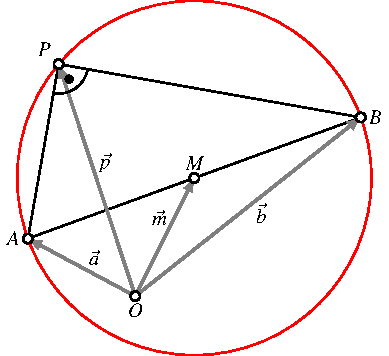
\includegraphics{4/images/thales.pdf}
\caption{Die Punkte $P$, von denen aus die Strecke $AB$ unter einem
rechten Winkel erscheint, bilden den Thaleskreis.
\label{thales-graphik}}
\end{figure}
Mit dem Skalarprodukt kann man ausdrücken, von welchen Punkten aus
eine Strecke $AB$ unter einem rechten Winkel gesehen wird.
Es ist dies die Menge der Punkte $P$ mit der Eigenschaft
\[
\overrightarrow{AP}\cdot\overrightarrow{BP}=0
\]
(Abbildung~\ref{thales-graphik}).
Unter Verwendung der Konvention, dass kleine Buchstaben für die
Ortsvektoren der Punkte mit entsprechenden Grossbuchstaben stehen, ist
dies gleichbedeutend mit
\[
(\vec p-\vec a)\cdot(\vec p-\vec b)=0
\]
Ausmultiplizieren und quadratisch ergänzen ergibt
\begin{align*}
\vec p^2-\vec p\cdot\vec b-\vec a\cdot\vec p+\vec a\cdot\vec b&=0
\\
\vec p^2-(\vec a+\vec b)\cdot \vec p+\vec a\cdot\vec b&=0
\\
\vec p^2-2\left(\frac{\vec a+\vec b}{2}\right)\cdot \vec p
+\left(\frac{\vec a+\vec b}{2}\right)^2
-\left(\frac{\vec a+\vec b}{2}\right)^2
+\vec a\cdot\vec b&=0
\\
\left(\vec p
-\frac{\vec a+\vec b}{2}\right)^2&=
\left(\frac{\vec a+\vec b}{2}\right)^2-\vec a\cdot \vec b
\\
&=
\frac{\vec a^2+2\vec a\cdot\vec b+\vec b^2-4\vec a\cdot \vec b}{4}
\\
&=
\frac{\vec a^2-2\vec a\cdot\vec b+\vec b^2}{4}
\\
\left(\vec p
-\frac{\vec a+\vec b}{2}\right)^2&=
\left(\frac{\vec a-\vec b}{2}\right)^2
\end{align*}
Diese Gleichung beschreibt einen Kreis um den Punkt $(\vec a+\vec b)/2$
mit dem Radius $|\vec a-\vec b|/2$.
Dies ist der Thaleskreis.

%
% Tangente in einem Punkt
%
\subsection{Tangente oder Tangentialebene in einem Punkt}
\begin{figure}
\centering
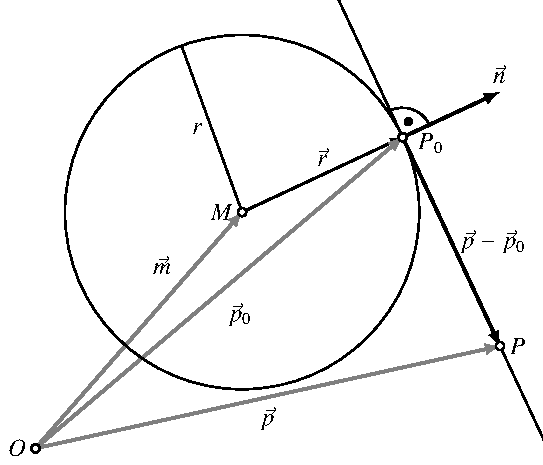
\includegraphics{4/images/tangente.pdf}
\caption{Tangente im Punkt $P_0$ an den Kreis um $M$ mit Radius $r$.
Der Vektor $\vec{p}-\vec{p}_0$ muss auf dem
Normalenvektor $\vec{n}$ senkrecht stehen, letzterer hat die Richtung
von $
%\overrightarrow{MP_0}=
\vec{p}_0-\vec{m}$.
\label{tangente-graphik}}
\end{figure}
Die Normale $\vec{n}$ auf einen Kreis ist immer parallel zum Radiusvektor
$\vec{r}$
(Abbildung~\ref{tangente-graphik}),
dasselbe gilt für eine Kugel.
Daher kann
man die Gleichung der Tangente in einem Punkt $P_0$ an einen Kreis
oder der Tangentialebene in einem Punkt der Kugel sofort angeben:
\begin{satz}\label{kugeltangentialebene}
Die Tangentialebene an eine Kugel mit Mittelpunktsortsvektor
$\vec m$ und Radius  $r$ im Punkt mit Ortsektor $\vec p_0$ ist
\begin{equation}
\{\vec p\;|\;
(\vec p-\vec p_0)\cdot(\vec p_0-\vec m)=0
\}
\label{eqn-kugeltangente}
\end{equation}
\end{satz}
Diese Form (\ref{eqn-kugeltangente}) ist noch nicht optimal, man kann den
Radius nicht direkt ablesen.

Man kann den Punkt $P$ aber auch dadurch charakterisieren, dass die
orthogonale Projektion des Vektors $\overrightarrow{MP}$ auf die
Gerade $MP_0$ immer die Länge $r$ haben muss. 
Mit dem Skalarprodukt kann man dies durch die Bedingung
\begin{equation}
(\vec{p}-\vec{m})\cdot \vec n = r
\label{skript:tangente1}
\end{equation}
ausdrücken.
Als Normaleneinheitsvektor kann man
\[
\vec{n}
=
\frac{\vec{p}_0-\vec{m}}{|\vec{p}_0-\vec{m}|}
= 
\frac{\vec{p}_0-\vec{m}}{r}
\]
verwenden.
Setzt man dies in \ref{skript:tangente1} ein, erhält man
\begin{align}
(\vec{p}-\vec{m})\cdot
\frac{\vec{p}_0-\vec{m}}{r}
&=
r
\notag
\\
\Rightarrow\qquad
(\vec{p}-\vec{m})\cdot
(\vec{p}_0-\vec{m})
&=
r^2.
\label{skript:tangente2}
\end{align}
Man erhält also die Tangentengleichung \ref{skript:tangente2}
aus der Kreisgleichung, indem man eine der Variablen $\vec{p}$
durch den Berührpunk $\vec{p}_0$ ersetzt.

Man kann die Gleichung \ref{skript:tangente2} auch wie folgt erhalten.
Für die Punkte $M$, $P$ und $P_0$ gelten einerseits die Tangentengleichung
\label{eqn-kugeltangente} und die Kreisgleichung für den Punkt $P_0$:
Addieren wir jedoch noch die Gleichung
der Kugel für den Vektor $\vec p_0$, erhalten wir
\begin{align*}
&\text{Tangentengleichung:}
&
(\vec p-\vec p_0)\cdot(\vec p_0-\vec m)&=0\\
&\text{Kreisgleichung für $P_0$:}
&
(\vec p_0-\vec m)\cdot(\vec p_0-\vec m)&=r^2.\\
\intertext{Addieren wir diese beiden Gleichungen, erhalten wir}
&&(\vec{p}-\vec{p}_0+\vec{p}_0-\vec m)\cdot(\vec p_0-\vec m)&=r^2
\\
&&(\vec p-\vec m)\cdot(\vec p_0-\vec m)&=r^2.
\end{align*}

%
% Tangente/Tangentialebene von einem Punkt aus
%
\subsection{Tangente von einem Punkt an einen Kreis}
\begin{figure}
\centering
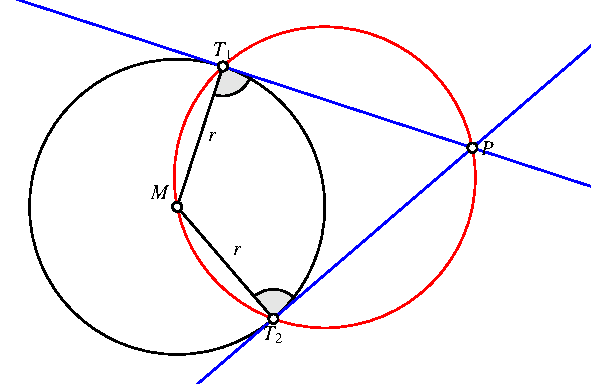
\includegraphics{4/images/tangentepunkt.pdf}
\caption{Tangente vom Punkt $P$ an den Kreis $K(M,r)$.
Die Berührpunkte $T_1$ und $T_2$ sind Schnittpunkte des Kreises mit
dem Thaleskreises (rot) über der Strecke $MP$.
\label{skript:ortho:tangentepunkt}}
\end{figure}
Es sind die Gleichungen der Tangenten an einen Kreis $K(M,r)$ zu finden,
welche durch den Punkt $P$ gehen.
Die klassische Konstruktion der
Elementargeometrie verlangt, dass über der Strecke $MP$ der
Thaleskreis gezeichnet wird, die Schnittpunkte des Thaleskreis mit
$K(M,r)$ sind die Berührpunkte der Tangenten
(Abbildung~\ref{skript:ortho:tangentepunkt}).

Die Tangenten sollen jetzt aber auf rein algebraische Art gefunden
werden.
Das Problem wäre im wesentlich gelöst, wenn der Berührpunkt $P_0$
mit Ortsvektor
$\vec p_0$ bekannt wäre.
Dieser muss natürlich auf dem Kreis liegen,
also
\[
(\vec p_0-\vec m)^2=r^2.
\]
Ausserdem muss der Punkt $P$ auf der Tangente im Punkt $P_0$ liegen,
also muss $\overrightarrow{MP_0}$ senkrecht auf $\overrightarrow{PP_0}$ stehen:
\begin{equation}
(\vec p_0-\vec m)\cdot(\vec p-\vec p_0)=0
\label{thalesbedingung}
\end{equation}
Damit haben wir zwei Gleichungen für die beiden unbekannten Koordinaten
von $P_0$ gefunden.
Im Allgemeinen werden sie die Bestimmung von $\vec p_0$
ermöglichen (Ausnahmen: $P$ im Inneren des Kreises).

Zur Lösung multiplizieren wir die zweite Gleichung noch aus
\begin{align*}
\vec p_0^2-\vec m\cdot\vec p_0-\vec p\cdot\vec p_0+\vec m\cdot\vec p&=0
\\
\vec p_0^2-\vec p_0\cdot (\vec m+\vec p)+\vec m\cdot\vec p&=0
\\
\vec p_0^2-2\vec p_0\cdot \left(\frac{\vec m+\vec p}{2}\right)+\vec m\cdot\vec p&=0
\\
\vec p_0^2-2\vec p_0\cdot \left(\frac{\vec m+\vec p}{2}\right)+
\left(\frac{\vec m+\vec p}2\right)^2
-\left(\frac{\vec m+\vec p}2\right)^2
+\vec m\cdot\vec p&=0
\\
\left(\vec p_0- \frac{\vec m+\vec p}{2}\right)^2
&=
\left(\frac{\vec m+\vec p}2\right)^2
-\vec m\cdot\vec p
\\
\left(\vec p_0- \frac{\vec m+\vec p}{2}\right)^2
&=
\left(\frac{\vec m-\vec p}2\right)^2
\end{align*}
Dies ist wieder ein Kreis mit Mittelpunkt $(\vec m+\vec p)/2$ und
Radius $|\vec m-\vec p|/2$, also wieder ein Thaleskreis.
Das ist natürlich nicht überraschend, die Bedingung (\ref{thalesbedingung})
ist ja nichts anderes als die Definition des Thaleskreises.
Die algebraische Rechnung macht also nichts anderes als die klassische
Konstruktion.

%
%  Reflexion eines Lichtstrahls und Ray-Tracing
%
\subsection{Reflexion eines Lichtstrahls}
\begin{figure}
\begin{center}
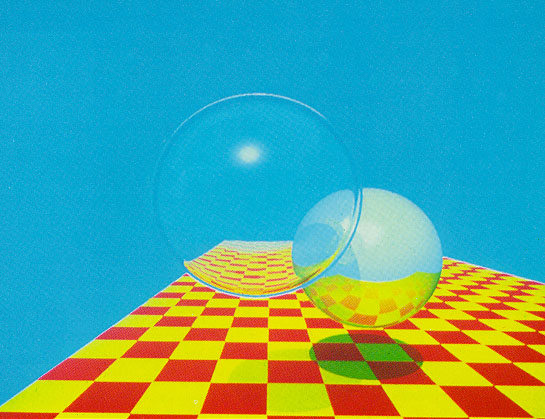
\includegraphics[width=1\hsize]{graphics/raytracing}
\end{center}
\caption{Mit Ray Tracing erzeugtes computergeneriertes Bild\label{raytracing}}
\end{figure}
Computergraphik-Effekte sind aus modernen Filmen nicht mehr wegzudenken.
Ganze Spielfilme wurden schon vollständig im Computer erzeugt.
Wie können die Bilder so realistisch wirken?

In Abschnitt \ref{spiegelung} haben wir gelernt, wie ein Vektor
gespiegelt wird.
Wir können also den Lichtstrahl, der in das Auge
des Beobachters einer Szene fällt, zurückverfolgen und seine Reflektion
an jeder beliebigen reflektierenden Fläche der Szene berechnen, bis wir bei
einer Lichtquelle oder einem nicht reflektierenden Objekt ankommen.
Die an diesem Punkt abgestrahlte Farbe ist dan jene, die der Beobachter
wahrnimmt.
Dieses Verfahren nennt man Ray Tracing.
Offenbar ist es sehr
aufwendig, denn Lichtstrahlen können nicht nur reflektiert, sondern auch
gestreut werden und sie können zum Beispiel durch Nebel oder Dunst abgeschwächt
werden.
Die Berechnung hochauflösender Szenen ist daher sehr aufwendig,
die Herstellung von CG-Filmen in Spielfilm-Länge, wie Pixar sie beispielsweise
produziert, benötigt die Rechenleistung grosser Computer-Cluster.

Die Berechnung der Reflexion an einer Kugel wie in Abbildung \ref{raytracing}
erfolgt nach folgendem Algorithmus:
\begin{enumerate}
\item Berechne den Durchstosspunkt des Lichtstrahles mit der reflektierenden
Kugeloberfläche wie in \ref{durchstosspunktkugel} beschrieben.
\item Berechnet die Normale im Durchstosspunkt gemäss Satz \ref{kugeltangentialebene}.
\item Berechne die gespiegelte Gerade gemäss Abschnitt \ref{spiegelung}.
\end{enumerate}
Dieses Verfahren wird jedoch nicht nur für die Computergraphik verwendet,
sondern auch in der Optik.
Spiegelteleskope bestehen aus gekrümmten Spiegeln.
Durch Berechnung der Strahlen kann man erfahren, welche Abbildungsqualität
man von dem Teleskop erwarten kann.

